\documentclass[11pt,a4paper]{article}
\usepackage[margin=2.6cm]{geometry}
\usepackage[T1]{fontenc}
\usepackage[utf8]{inputenc}
\usepackage{lmodern}
\usepackage{microtype}
\usepackage{booktabs}
\usepackage{longtable}
\usepackage{graphicx}
\usepackage{amsmath}
\usepackage[hidelinks]{hyperref}
\usepackage{caption}
\captionsetup{font=small,labelfont=bf,width=.92\textwidth}
\usepackage{setspace}
\setstretch{1.08}
\graphicspath{{../figures/}}
\newcommand{\nCompanies}{99}
\newcommand{\nFilings}{1,792}
\newcommand{\nPairs}{1,690}
\newcommand{\nPairsIA}{1,560}
\newcommand{\nPairsVII}{1,297}
\newcommand{\nMonths}{211}
\newcommand{\sampleStart}{March 2009}
\newcommand{\sampleEnd}{September 2026}
\newcommand{\spySharpe}{1.02}
\newcommand{\legSize}{19}
\newcommand{\legMin}{14}
\newcommand{\turnover}{3.2}
\newcommand{\LSmean}{-0.92}
\newcommand{\LSvol}{8.46}
\newcommand{\LSsharpe}{-0.11}
\newcommand{\LSdd}{-33.1}
\newcommand{\LSsharpeLo}{-0.56}
\newcommand{\LSsharpeHi}{0.38}
\newcommand{\LSalphaCAPM}{-0.68}
\newcommand{\LStCAPM}{-0.37}
\newcommand{\LSalphaFFthree}{-0.42}
\newcommand{\LStFFthree}{-0.23}
\newcommand{\LSalphaFFfive}{-0.93}
\newcommand{\LStFFfive}{-0.49}
\newcommand{\LSnetmean}{-1.24}
\newcommand{\LSnetvol}{8.49}
\newcommand{\LSnetsharpe}{-0.15}
\newcommand{\LSnetdd}{-34.6}
\newcommand{\LSnetsharpeLo}{-0.58}
\newcommand{\LSnetsharpeHi}{0.34}
\newcommand{\LSnetalphaCAPM}{-1.00}
\newcommand{\LSnettCAPM}{-0.53}
\newcommand{\LSnetalphaFFthree}{-0.73}
\newcommand{\LSnettFFthree}{-0.40}
\newcommand{\LSnetalphaFFfive}{-1.25}
\newcommand{\LSnettFFfive}{-0.65}
\newcommand{\nTrials}{54}
\newcommand{\nTrialsPositive}{17}
\newcommand{\nTrialsSig}{8}
\newcommand{\nTrialsSigNeg}{8}
\newcommand{\bestTrial}{cos\_1a$\mid$q10$\mid$lag2}
\newcommand{\bestSharpe}{0.54}
\newcommand{\medianSharpe}{-0.05}
\newcommand{\emaxRaw}{0.80}
\newcommand{\dsrRaw}{0.13}
\newcommand{\nEff}{4.2}
\newcommand{\emaxEff}{0.37}
\newcommand{\dsrEff}{0.76}
\newcommand{\pbo}{0.08}
\newcommand{\probOOSloss}{0.21}
\newcommand{\cscvCombos}{12,870}
\newcommand{\nObsCommon}{201}
\newcommand{\bestOwnAlpha}{4.30}
\newcommand{\bestOwnT}{1.34}
\newcommand{\bestOwnDD}{-41}
\newcommand{\worstTrial}{jac\_7$\mid$q5$\mid$lag0}
\newcommand{\worstMean}{-10.0}
\newcommand{\worstAlpha}{-9.3}
\newcommand{\worstT}{-2.57}
\newcommand{\worstDD}{-85}
\newcommand{\nPlacebo}{200}
\newcommand{\placeboPct}{34}
\newcommand{\placeboSd}{0.25}
\newcommand{\placeboLo}{-0.42}
\newcommand{\placeboHi}{0.40}
\newcommand{\placeboAbsT}{6}
\newcommand{\placeboBestPct}{99.5}
\newcommand{\carLS}{-1.8}
\newcommand{\carLSt}{-0.60}
\newcommand{\carQlow}{4.2}
\newcommand{\carQhigh}{2.4}
\newcommand{\cosMedian}{0.996}
\newcommand{\cosQone}{0.994}
\newcommand{\cosQthree}{0.998}
\newcommand{\jacMedian}{0.88}
\newcommand{\jacQone}{0.85}
\newcommand{\jacQthree}{0.91}
\newcommand{\jacFirst}{0.84}
\newcommand{\jacLast}{0.91}
\newcommand{\shareMissingVII}{23}
\newcommand{\shareMissingIA}{8}


\title{\textbf{Lazy Prices on the S\&P~100:\\a replication and an overfitting audit}}
\author{Ignacio Queipo de Llano\thanks{Code, data and this note: \url{https://github.com/iqueipopg/lazy-prices}. All numbers in the text are macros generated from the result files by \texttt{python -m lazyprices.report}.}}
\date{September 2026}

\begin{document}
\maketitle

\begin{abstract}
\noindent Cohen, Malloy and Nguyen (2020) show that firms whose annual report changes little from one year to the next outperform firms whose report changes a lot, and that a long-short portfolio on this signal earned 30 to 60 basis points a month on the CRSP universe from 1995 to 2014. I replicate the strategy on the current S\&P~100 with free data (\nFilings{} 10-K filings from EDGAR, yfinance prices, Fama-French factors) over \sampleStart{} to \sampleEnd. The long-short portfolio earns \LSmean\% a year with an FF5+MOM alpha of \LSalphaFFfive\% ($t = \LStFFfive$); the twelve-month event-time abnormal return is \carLS\% ($t = \carLSt$); the within-cohort rank correlation between text change and forward return is indistinguishable from zero for every measure. Searching over \nTrials{} variants produces a best annualised Sharpe of \bestSharpe, but the deflated Sharpe ratio of that winner is \dsrRaw{} and its Sharpe sits at the \placeboBestPct th percentile of a placebo distribution obtained by shuffling scores within cohorts. On this universe and period there is no detectable effect. The note documents why that is the expected outcome given the sample and how the tools of Bailey and L\'opez de Prado keep the best of \nTrials{} backtests from being reported as a finding.
\end{abstract}

\section{Introduction}

\emph{Lazy Prices} argues that annual reports are read by few and changed by fewer: when a firm rewrites large parts of its 10-K, the rewrite usually carries bad news, concentrated in the risk factors (Item 1A) and the management discussion (Item 7), and the market absorbs it slowly. The authors measure the change with four similarity measures between consecutive 10-Ks and 10-Qs, sort firms into quintiles, and find that a portfolio long ``non-changers'' and short ``changers'' earns 30 to 60 basis points a month of abnormal return over the following year, with the effect concentrated in the months after the filing.

This note asks a narrow question: does the signal show up in the largest and most scrutinised US companies, using only public, free data? The answer is no, and the interesting part of the exercise is establishing that the ``no'' is robust to the researcher's own degrees of freedom. Section~\ref{sec:data} describes the data and its limitations, Section~\ref{sec:method} the construction, Section~\ref{sec:results} the results, Section~\ref{sec:overfit} the selection-bias audit and Section~\ref{sec:conclusion} what I would conclude.

\section{Data}\label{sec:data}

\paragraph{Universe.} The \nCompanies{} companies of the S\&P~100 as of September 2026, identified by CIK. This is a \emph{current} list, so every firm in it survived and grew into the index; firms that were members in 2010 and later shrank, were acquired or failed are absent. Five companies changed CIK after a holding-company reorganisation (Exxon Mobil, Alphabet, Disney, BlackRock, Medtronic); the predecessor registrant's filings are attributed to the current ticker. Companies listed later (AbbVie, Meta, PayPal, Uber, Palantir and others) enter when their second 10-K exists.

\paragraph{Filings.} \nFilings{} original 10-K filings for fiscal years 2007 to 2025 (10-K/A amendments excluded), downloaded from the EDGAR submissions index and Archives with the required identifying \texttt{User-Agent}, at most eight requests a second and a local cache. FY2007 is used only as the predecessor of FY2008. The primary document is converted to plain text (inline-XBRL hidden blocks and CSS-hidden elements dropped, line breaks only at block elements so that headings are not split). Items 1A and 7 are located by pairing each ``Item 1A. Risk Factors'' / ``Item 7. Management's Discussion'' heading with the next ``Item 1B/2'' / ``Item 7A/8'' heading and keeping the longest span; table-of-contents entries and cross-references produce short spans and lose. Extractions shorter than 2,000 characters are treated as missing: Item 7 is missing in \shareMissingVII\% of pairs (banks and some industrials incorporate the MD\&A by reference to the annual report exhibit) and Item 1A in \shareMissingIA\%.

\paragraph{Prices and factors.} Adjusted daily closes from yfinance for the \nCompanies{} tickers and SPY from January 2007; daily Fama-French five factors and momentum from the Kenneth French Data Library, compounded within calendar months.

\section{Method}\label{sec:method}

\paragraph{Similarity.} For each pair of consecutive 10-Ks of the same company (report dates 270 to 500 days apart), and for the full document, Item 1A and Item 7, two measures are computed on lower-case alphabetic tokens of at least two letters: cosine similarity between TF-IDF vectors and Jaccard similarity between the sets of distinct terms. The inverse document frequency is computed \emph{point in time} from all 10-Ks filed in months before the later filing, so a score never depends on documents that were not yet public. This yields \nPairs{} pairs (\nPairsIA{} with Item 1A, \nPairsVII{} with Item 7).

Before any portfolio is formed, the first result is descriptive: cosine similarity on the full document is nearly saturated, with a median of \cosMedian{} and an interquartile range of \cosQone{} to \cosQthree. Annual reports of the largest US companies are long and mostly boilerplate, so the sort is made on the third decimal. Jaccard has more dispersion (median \jacMedian, IQR \jacQone{} to \jacQthree), and its median rose from \jacFirst{} in FY2008 to \jacLast{} in FY2025 (Figure~\ref{fig:sim}).

\begin{figure}[htbp]\centering
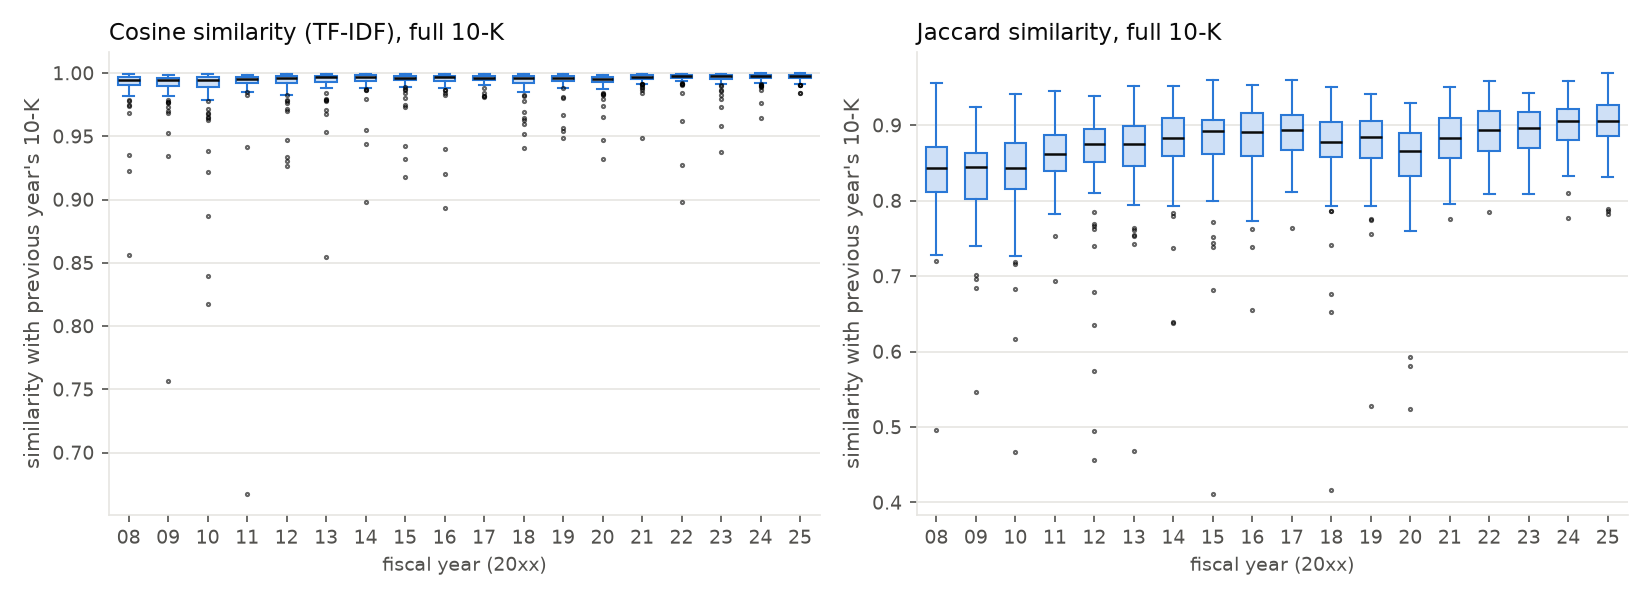
\includegraphics[width=\textwidth]{similarity_by_year.png}
\caption{Similarity between consecutive 10-Ks of the same company, by fiscal year.}\label{fig:sim}
\end{figure}

\paragraph{Portfolios.} Filings are grouped into fiscal-year cohorts (the calendar year in which the reporting period ends; periods ending in the first two weeks of January belong to the previous year). Within each cohort, companies are sorted on the score into quintiles; Q5 holds the least-changed reports. A stock enters its quintile portfolio at the close of the first trading day of the month after its filing date and is held for twelve months, so the portfolio at any date averages the overlapping annual cohorts. Portfolios are equal-weighted; the long-short portfolio is Q5 minus Q1 and is defined only when both legs hold at least five stocks (about \legSize{} on average, minimum \legMin). Transaction costs are 10 basis points per unit of one-way turnover on each leg; realised turnover is \turnover{} per year for the two legs together.

Ranking within a fiscal-year cohort means that an early filer's quintile depends on scores of firms filing later in the same season. Prices are never used before the filing date (the test suite checks the formation calendar), but the ranking is not strictly real time; a fully point-in-time variant that ranks each filing against the trailing twelve months of filings is reported as a robustness check.

\paragraph{Evaluation.} Monthly returns of each quintile (in excess of the risk-free rate) and of the long-short portfolio are regressed on the CAPM, Fama-French three-factor and Fama-French five-factor plus momentum models with Newey-West standard errors (automatic lag $\lfloor 4(T/100)^{2/9}\rfloor = 4$). Sharpe ratios are annualised from monthly returns; a circular block bootstrap (blocks of six months, 2,000 draws) gives their confidence interval. Two model-free checks complement the portfolios: the cumulative market-adjusted return of each quintile by event month after formation, and the within-cohort Spearman correlation between the score and the twelve-month forward return, averaged across cohorts.

\paragraph{Variants and selection bias.} The grid of variants is measure (cosine, Jaccard) $\times$ section (full, Item 1A, Item 7) $\times$ groups (terciles, quintiles, deciles) $\times$ formation lag (0, 1, 2 months): \nTrials{} trials. Their long-short returns on the common sample (\nObsCommon{} months) feed the deflated Sharpe ratio of Bailey and L\'opez de Prado (2014), with the effective number of trials estimated from the participation ratio of the trial correlation matrix, and the probability of backtest overfitting via combinatorially symmetric cross-validation (Bailey et al., 2017; $S = 16$, \cscvCombos{} partitions). A placebo re-runs the main specification \nPlacebo{} times with scores permuted within cohorts, which preserves every breakpoint and only breaks the link between text and company.

\section{Results}\label{sec:results}

\subsection{Main specification}

\begin{table}[htbp]\centering\small
\caption{Long-short portfolio (Q5 minus Q1), main specification: cosine TF-IDF on the full 10-K, quintiles within fiscal-year cohorts, formation the month after filing, twelve-month hold. 211 months, March 2009 to September 2026. Newey-West $t$-statistics with 4 lags.}\label{tab:main}
\begin{tabular}{lrr}\toprule
 & Gross & Net of 10 bp per unit turnover \\ \midrule
Mean return (\% p.a.) & -0.92 & -1.24 \\
Volatility (\% p.a.) & 8.46 & 8.49 \\
Sharpe ratio & -0.11 & -0.15 \\
Sharpe ratio, 95\% bootstrap interval & [-0.56, 0.38] & [-0.58, 0.34] \\
Maximum drawdown (\%) & -33.10 & -34.65 \\
CAPM alpha (\% p.a.), $t$-statistic & -0.68 (-0.37) & -1.00 (-0.53) \\
FF3 alpha (\% p.a.), $t$-statistic & -0.42 (-0.23) & -0.73 (-0.40) \\
FF5+MOM alpha (\% p.a.), $t$-statistic & -0.93 (-0.49) & -1.25 (-0.65) \\
\bottomrule\end{tabular}\end{table}


The long-short portfolio returns \LSmean\% a year before costs with a Sharpe ratio of \LSsharpe{} (bootstrap 95\% interval $[\LSsharpeLo, \LSsharpeHi]$) and an FF5+MOM alpha of \LSalphaFFfive\% ($t=\LStFFfive$); the CAPM and FF3 alphas are \LSalphaCAPM\% ($t=\LStCAPM$) and \LSalphaFFthree\% ($t=\LStFFthree$). Costs subtract about \turnover{} $\times$ 10 bp a year. SPY over the same months had a Sharpe ratio of \spySharpe. Figure~\ref{fig:cum} shows the cumulative return.

\begin{figure}[htbp]\centering
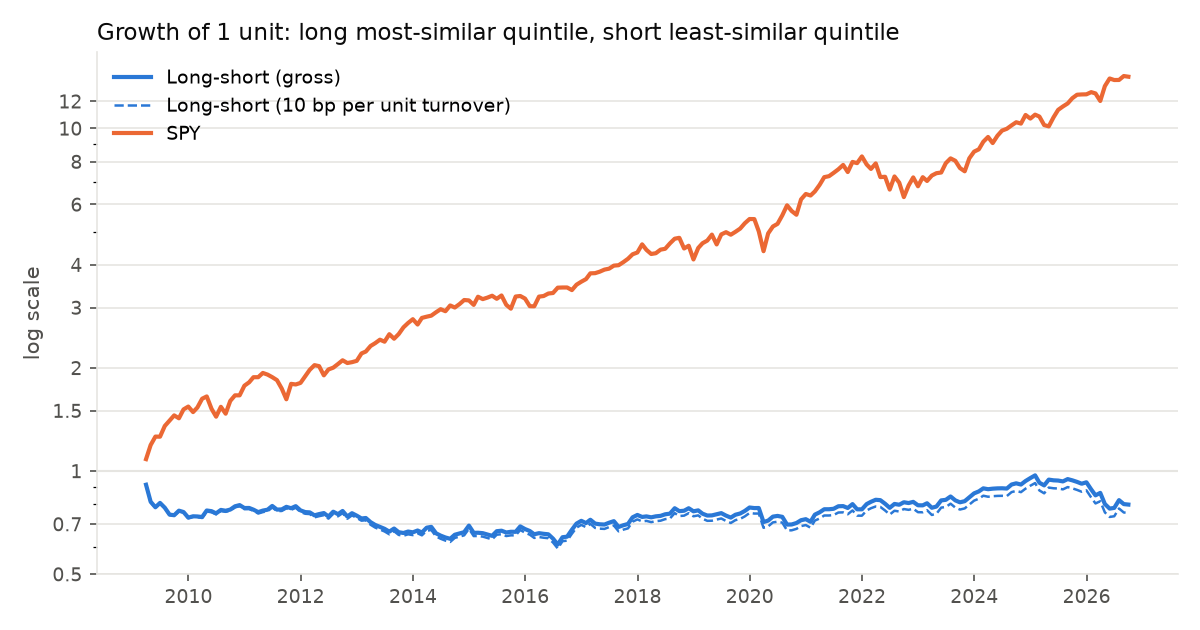
\includegraphics[width=.9\textwidth]{cumulative_long_short_vs_spy.png}
\caption{Growth of one unit in the long-short portfolio, gross and net of costs, and in SPY.}\label{fig:cum}
\end{figure}

\subsection{Quintiles}

\begin{table}[htbp]\centering\small
\caption{Quintile portfolios, monthly returns in excess of the risk-free rate. Mean, volatility, drawdown and alphas in percent per year.}\label{tab:quintiles}
\begin{tabular}{lrrrrrrr}\toprule
Quintile & Mean & Vol & Sharpe & Max DD & CAPM $\alpha$ ($t$) & FF3 $\alpha$ ($t$) & FF5+MOM $\alpha$ ($t$) \\ \midrule
Q1 (most change) & 19.4 & 16.5 & 1.17 & -23.0 & 4.42 (3.00) & 4.18 (2.93) & 4.54 (3.15) \\
Q2 & 22.3 & 16.3 & 1.37 & -21.5 & 7.48 (4.24) & 7.36 (4.33) & 7.73 (4.62) \\
Q3 & 16.2 & 14.6 & 1.10 & -21.4 & 2.84 (1.89) & 2.34 (1.65) & 2.20 (1.54) \\
Q4 & 19.0 & 15.3 & 1.24 & -26.4 & 4.61 (4.34) & 4.39 (4.09) & 4.60 (4.69) \\
Q5 (least change) & 18.6 & 16.2 & 1.15 & -28.5 & 3.66 (2.26) & 3.67 (3.31) & 3.55 (3.18) \\
\bottomrule\end{tabular}\end{table}


There is no monotonic pattern across quintiles (Table~\ref{tab:quintiles}, Figure~\ref{fig:quint}). Every quintile has a positive alpha of 2\% to 8\% a year. That is not a property of the strategy: it is the survivorship signature of a universe chosen after the fact, and it affects both legs in the same direction.

\begin{figure}[htbp]\centering
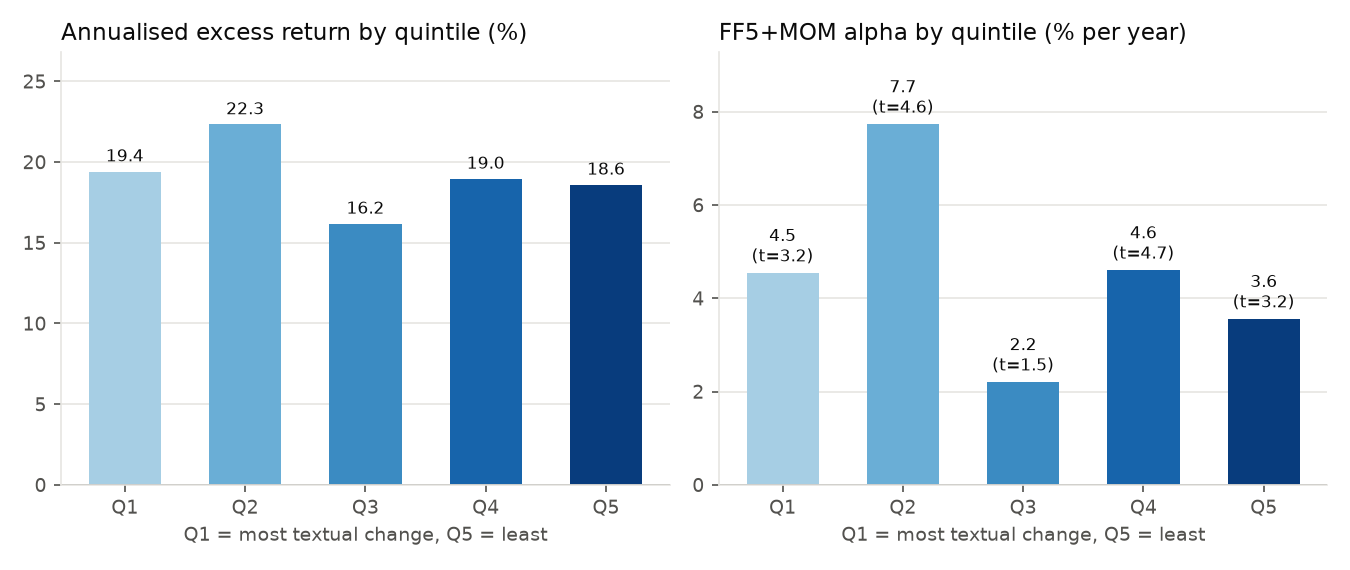
\includegraphics[width=\textwidth]{quintile_returns.png}
\caption{Annualised excess return and FF5+MOM alpha by quintile.}\label{fig:quint}
\end{figure}

\subsection{Event time}

\begin{table}[htbp]\centering\small
\caption{Cumulative market-adjusted (minus SPY) return in percent by event month after formation, averaged first within and then across fiscal-year cohorts; the standard error treats each cohort as one observation.}\label{tab:eventtime}
\begin{tabular}{lrrrrr}\toprule
Month & Q1 CAR & Q5 CAR & Q5 $-$ Q1 & s.e. & Filings \\ \midrule
1 & 0.61 & -1.04 & -1.65 & 0.58 & 1690 \\
3 & 2.10 & -0.85 & -2.95 & 1.39 & 1690 \\
6 & 2.19 & -0.34 & -2.52 & 1.57 & 1688 \\
9 & 2.99 & 0.30 & -2.69 & 3.09 & 1614 \\
12 & 4.18 & 2.43 & -1.75 & 2.92 & 1603 \\
\bottomrule\end{tabular}\end{table}


The paper's central figure is the cumulative abnormal return in the months after the filing. Here (Table~\ref{tab:eventtime}, Figure~\ref{fig:event}) the least-changed quintile accumulates \carQhigh\% over twelve months against SPY and the most-changed quintile \carQlow\%; the difference is \carLS\% with a $t$-statistic of \carLSt{} when each cohort is treated as one observation. The sign is opposite to the paper and the magnitude is inside the noise.

\begin{figure}[htbp]\centering
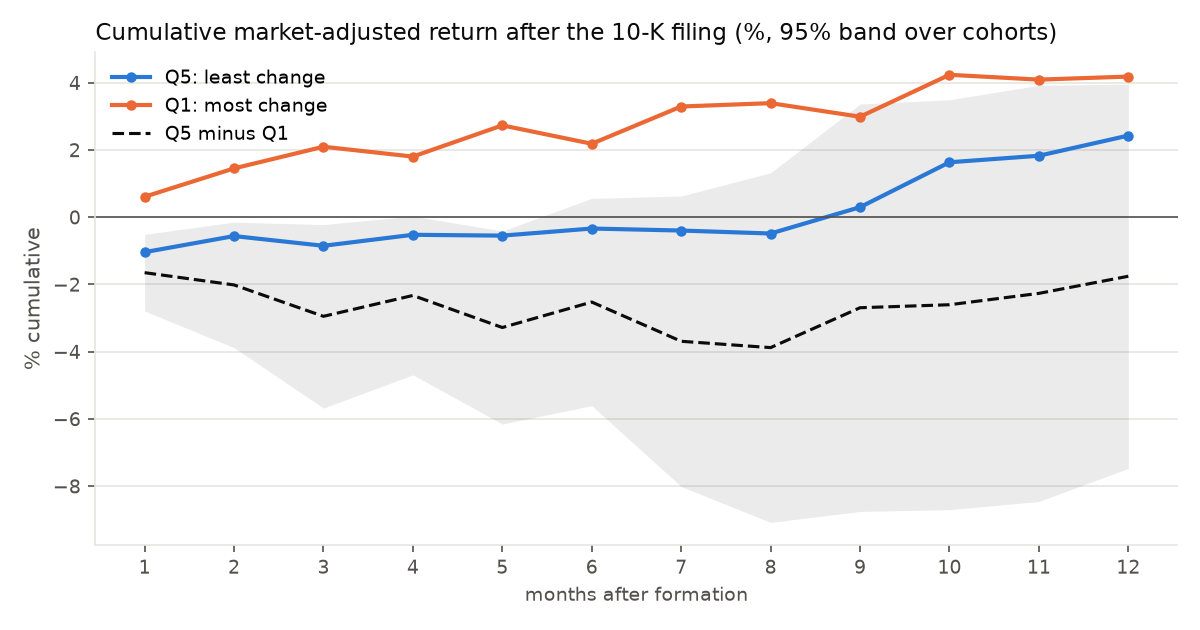
\includegraphics[width=.9\textwidth]{event_time_car.png}
\caption{Cumulative market-adjusted return by event month after formation; band is $\pm 1.96$ standard errors over cohorts for the difference.}\label{fig:event}
\end{figure}

\subsection{Robustness and a model-free check}

\begin{table}[htbp]\centering\small
\caption{Robustness of the main specification.}\label{tab:robustness}
\begin{tabular}{lrrrr}\toprule
Specification & Months & Mean (\% p.a.) & Sharpe & FF5+MOM $\alpha$ ($t$) \\ \midrule
main & 211 & -0.92 & -0.11 & -0.93 (-0.49) \\
trailing-window ranking (point-in-time) & 214 & -1.48 & -0.15 & -2.73 (-0.87) \\
main, 2009-2016 & 94 & -3.85 & -0.43 & -1.27 (-0.52) \\
main, 2017-2026 & 117 & 1.44 & 0.18 & 2.09 (1.09) \\
\bottomrule\end{tabular}\end{table}

\begin{table}[htbp]\centering\small
\caption{Spearman correlation, within each fiscal-year cohort, between the similarity score and the twelve-month return after formation; time-series mean over cohorts and its $t$-statistic.}\label{tab:rankcorr}
\begin{tabular}{lrrr}\toprule
Score & Mean rank correlation & $t$-statistic & Cohorts positive \\ \midrule
Cosine, full document & 0.035 & 1.14 & 12 of 17 \\
Cosine, Item 1A & 0.041 & 1.00 & 11 of 17 \\
Cosine, Item 7 & 0.006 & 0.18 & 10 of 17 \\
Jaccard, full document & 0.034 & 0.93 & 11 of 17 \\
Jaccard, Item 1A & -0.006 & -0.15 & 9 of 17 \\
Jaccard, Item 7 & -0.010 & -0.30 & 10 of 17 \\
\bottomrule\end{tabular}\end{table}


The fully point-in-time ranking, and each half of the sample, give the same answer (Table~\ref{tab:robustness}). The rank correlations in Table~\ref{tab:rankcorr} have the paper's sign for the full document and for cosine on Item 1A but are three to four hundredths in magnitude with $t$-statistics near one.

\section{Overfitting audit}\label{sec:overfit}

\begin{table}[htbp]\centering\small
\caption{Selection-bias corrections and placebo test.}\label{tab:overfitting}
\begin{tabular}{lr}\toprule
 & Value \\ \midrule
Variants tried & 54 \\
Variants with a positive Sharpe ratio & 17 \\
Variants with $|t| > 2$ on the FF5+MOM alpha & 8 (all negative) \\
Best variant on the common sample & \texttt{cos\_1a$\mid$q10$\mid$lag2} \\
Annualised Sharpe, best / median variant & 0.54 / -0.05 \\
E[max Sharpe] of $N$ zero-skill trials, raw $N$ & 0.80 \\
\textbf{Deflated Sharpe ratio, raw $N$} & \textbf{0.13} \\
Effective number of trials (participation ratio) & 4.2 \\
E[max Sharpe], effective $N$ & 0.37 \\
Deflated Sharpe ratio, effective $N$ & 0.76 \\
PBO (CSCV, $S=16$, 12,870 partitions) & 0.08 \\
P[out-of-sample loss of the in-sample winner] & 0.21 \\
Placebo: share of 200 shuffles with Sharpe below the actual strategy & 0.34 \\
Placebo: standard deviation of the Sharpe ratio across shuffles & 0.25 \\
Placebo: share of shuffles with $|t| > 2$ & 0.06 \\
\bottomrule\end{tabular}\end{table}


Of the \nTrials{} variants, \nTrialsPositive{} have a positive Sharpe ratio and \nTrialsSig{} have $|t| > 2$ on the FF5+MOM alpha; all \nTrialsSigNeg{} of the latter are Item 7 variants with a \emph{negative} alpha, that is, the opposite sign to the paper. The best variant on the common sample is \texttt{\bestTrial} with an annualised Sharpe of \bestSharpe{} (on its own full sample: alpha \bestOwnAlpha\%, $t = \bestOwnT$, maximum drawdown \bestOwnDD\%). Reported alone it would look like a modest finding. Against the expected maximum Sharpe of \nTrials{} zero-skill trials with the observed dispersion, \emaxRaw, its deflated Sharpe ratio is \dsrRaw; even against the lenient null of \nEff{} independent trials (expected maximum \emaxEff) it is \dsrEff, below the 0.95 certification threshold (Figure~\ref{fig:dsr}).

\begin{figure}[htbp]\centering
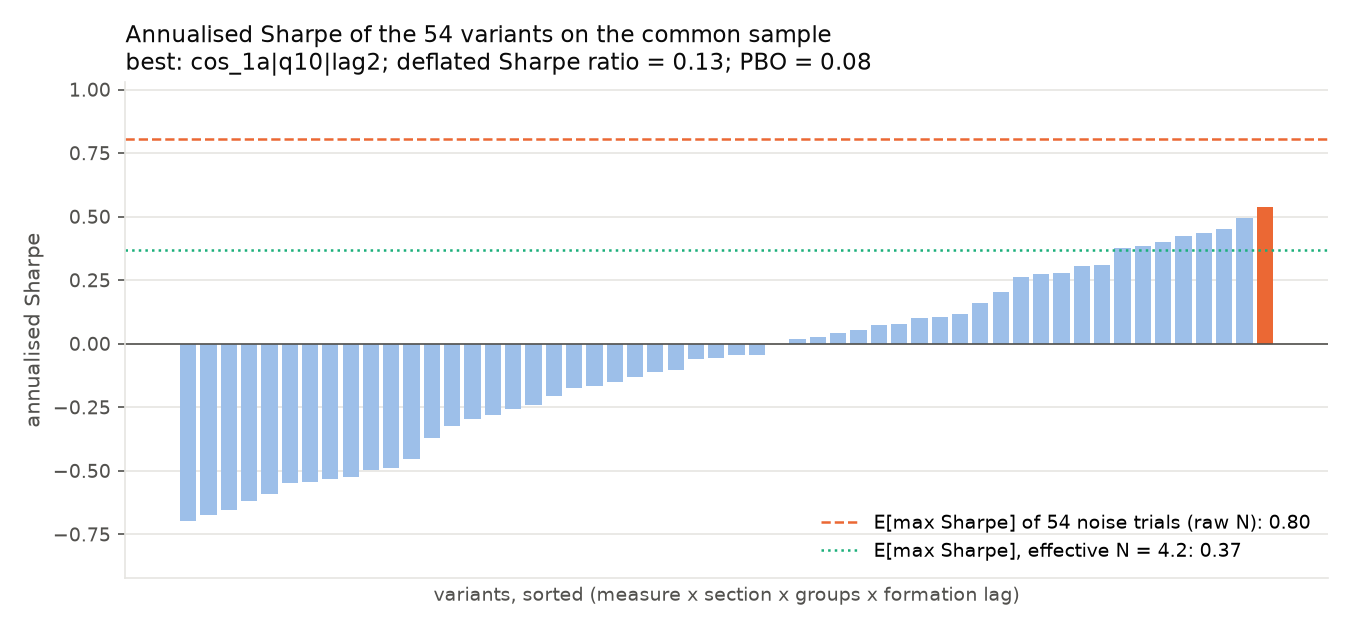
\includegraphics[width=\textwidth]{dsr_trials.png}
\caption{Annualised Sharpe ratio of every variant on the common sample; dashed lines are the expected maximum Sharpe of $N$ zero-skill trials for the raw and effective $N$.}\label{fig:dsr}
\end{figure}

The probability of backtest overfitting is low, \pbo, and should not be read as reassurance. CSCV asks whether the in-sample winner keeps ranking well \emph{relative to the other variants} out of sample. It does, because the Item 7 variants are consistently the worst and the Item 1A cosine variants consistently the least bad; relative rankings are stable. PBO measures overfitting within the search, not whether the winner is profitable: the in-sample winner still loses money out of sample in \probOOSloss{} of the partitions.

The placebo (Figure~\ref{fig:placebo}) shows what the machinery produces when the text carries no information. Shuffling scores within cohorts \nPlacebo{} times gives long-short Sharpe ratios with a standard deviation of \placeboSd{} and a 5th to 95th percentile range of \placeboLo{} to \placeboHi; the actual strategy sits at the \placeboPct th percentile, and \placeboAbsT\% of shuffles produce an alpha with $|t|>2$ on their own, about the nominal size. The best of the \nTrials{} variants sits at the \placeboBestPct th percentile of this single-specification null, which is exactly why the comparison must be made against the maximum of $N$ trials, as the DSR does, and not against one draw.

\begin{figure}[htbp]\centering
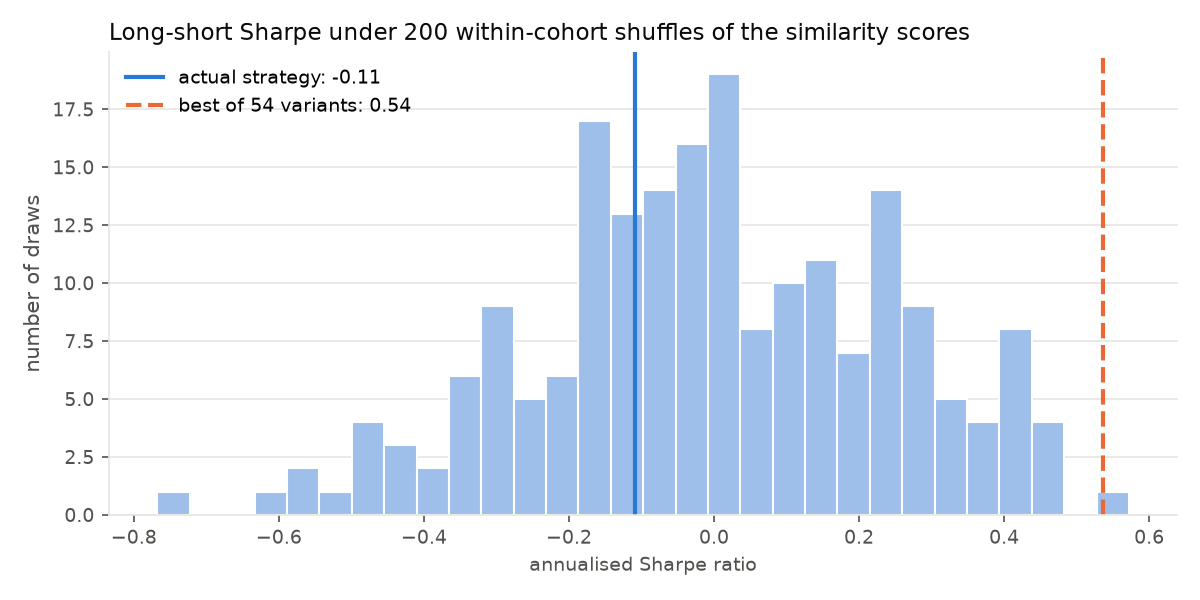
\includegraphics[width=.9\textwidth]{placebo_sharpe.png}
\caption{Distribution of the long-short Sharpe ratio when similarity scores are permuted within fiscal-year cohorts.}\label{fig:placebo}
\end{figure}

The worst variant, \texttt{\worstTrial}, loses \worstMean\% a year (alpha \worstAlpha\%, $t=\worstT$, drawdown \worstDD\%). Among these firms the ones that rewrote their MD\&A the most did better over the following year. The rank correlations for Item 7 are zero, so this is a tail effect in the extreme groups of a subsample that excludes the banks whose MD\&A is incorporated by reference. With \nTrials{} correlated trials, \nTrialsSig{} of them at $|t|>2$ in the wrong direction is what dispersion looks like, not evidence of a reverse effect.

\section{What I would conclude}\label{sec:conclusion}

\begin{enumerate}
\item On the current S\&P~100 from \sampleStart{} to \sampleEnd{} there is no detectable Lazy Prices effect. The main specification's alpha is slightly negative and indistinguishable from zero under every factor model, with or without costs; the event-time and rank-correlation checks agree.
\item This is not a rejection of the paper. Its effect is estimated on thousands of firms over a period before the idea was published. Here the universe is 100 of the most scrutinised companies in the world, selected after the fact for having survived, in a period after publication. A null in this setting is consistent with the paper's own mechanism: slow attention matters least where attention is greatest.
\item The measurement is weak for this universe. Cosine similarity on the full document is essentially one for every firm every year. Item-level measures help a little but are not always extractable.
\item The best of \nTrials{} variants has a Sharpe ratio of \bestSharpe{} and a $t$-statistic above one. The deflated Sharpe ratio (\dsrRaw) and the placebo say it is what the luckiest of \nTrials{} noise trials would show. Reporting the grid, the DSR and the placebo alongside the winner is the difference between a backtest and a result.
\end{enumerate}

\paragraph{Limitations and next steps.} A historical constituent list would remove the survivorship bias; extending the universe to the S\&P~500 or to all of EDGAR for a subperiod would give the test power; adding 10-Qs would triple the number of signals as in the paper. None changes the conclusion of this note, which is about what can and cannot be learned from 100 large caps.

\section*{References}
\begin{itemize}\setlength\itemsep{2pt}
\item Bailey, D.~H. and L\'opez de Prado, M. (2014). The Deflated Sharpe Ratio: Correcting for Selection Bias, Backtest Overfitting and Non-Normality. \emph{Journal of Portfolio Management}, 40(5), 94--107.
\item Bailey, D.~H., Borwein, J.~M., L\'opez de Prado, M. and Zhu, Q.~J. (2017). The Probability of Backtest Overfitting. \emph{Journal of Computational Finance}, 20(4), 39--69.
\item Cohen, L., Malloy, C. and Nguyen, Q. (2020). Lazy Prices. \emph{Journal of Finance}, 75(3), 1371--1415.
\item Fama, E.~F. and French, K.~R. (2015). A five-factor asset pricing model. \emph{Journal of Financial Economics}, 116(1), 1--22.
\item Newey, W.~K. and West, K.~D. (1994). Automatic Lag Selection in Covariance Matrix Estimation. \emph{Review of Economic Studies}, 61(4), 631--653.
\end{itemize}

\appendix
\section{All variants}
\begin{longtable}{lrrrrr}
\caption{All variants, sorted by annualised Sharpe ratio of the long-short portfolio on each variant's own sample. Alphas in percent per year (FF5+MOM, Newey-West $t$).}\label{tab:trials}\\
\toprule Variant & Months & Mean (\% p.a.) & Sharpe & $\alpha$ & $t$ \\ \midrule \endfirsthead
\toprule Variant & Months & Mean (\% p.a.) & Sharpe & $\alpha$ & $t$ \\ \midrule \endhead
\bottomrule \endfoot
\texttt{cos\_full$\mid$q10$\mid$lag2} & 209 & 4.19 & 0.43 & 3.03 & 1.34 \\
\texttt{cos\_1a$\mid$q5$\mid$lag2} & 209 & 3.62 & 0.43 & 3.17 & 1.70 \\
\texttt{cos\_1a$\mid$q10$\mid$lag2} & 209 & 5.25 & 0.41 & 4.30 & 1.34 \\
\texttt{cos\_1a$\mid$q5$\mid$lag1} & 210 & 3.40 & 0.38 & 3.12 & 1.60 \\
\texttt{cos\_full$\mid$q10$\mid$lag1} & 210 & 3.42 & 0.33 & 2.27 & 0.97 \\
\texttt{cos\_1a$\mid$q5$\mid$lag0} & 211 & 2.84 & 0.31 & 2.46 & 1.27 \\
\texttt{cos\_1a$\mid$q10$\mid$lag0} & 211 & 4.08 & 0.31 & 3.40 & 1.16 \\
\texttt{cos\_1a$\mid$q10$\mid$lag1} & 210 & 3.91 & 0.30 & 3.32 & 1.09 \\
\texttt{cos\_1a$\mid$q3$\mid$lag2} & 210 & 1.56 & 0.22 & 0.98 & 0.69 \\
\texttt{cos\_full$\mid$q10$\mid$lag0} & 211 & 2.23 & 0.20 & 0.89 & 0.33 \\
\texttt{cos\_1a$\mid$q3$\mid$lag0} & 212 & 1.35 & 0.17 & 1.01 & 0.63 \\
\texttt{jac\_full$\mid$q3$\mid$lag2} & 212 & 1.15 & 0.16 & 0.84 & 0.50 \\
\texttt{cos\_full$\mid$q5$\mid$lag2} & 209 & 1.04 & 0.15 & 0.89 & 0.58 \\
\texttt{cos\_full$\mid$q5$\mid$lag1} & 210 & 0.77 & 0.10 & 0.77 & 0.46 \\
\texttt{cos\_1a$\mid$q3$\mid$lag1} & 211 & 0.66 & 0.08 & 0.19 & 0.11 \\
\texttt{jac\_1a$\mid$q5$\mid$lag2} & 209 & 0.52 & 0.06 & 0.44 & 0.21 \\
\texttt{jac\_1a$\mid$q5$\mid$lag1} & 210 & 0.31 & 0.04 & 0.49 & 0.23 \\
\texttt{jac\_full$\mid$q5$\mid$lag1} & 210 & -0.01 & -0.00 & 0.56 & 0.29 \\
\texttt{jac\_full$\mid$q5$\mid$lag2} & 209 & -0.03 & -0.00 & 0.10 & 0.05 \\
\texttt{jac\_1a$\mid$q5$\mid$lag0} & 211 & -0.05 & -0.01 & -0.01 & -0.00 \\
\texttt{jac\_full$\mid$q3$\mid$lag1} & 213 & -0.23 & -0.03 & -0.53 & -0.23 \\
\texttt{jac\_full$\mid$q10$\mid$lag0} & 209 & -0.53 & -0.05 & 1.24 & 0.56 \\
\texttt{jac\_full$\mid$q10$\mid$lag2} & 207 & -0.51 & -0.05 & 0.28 & 0.12 \\
\texttt{jac\_full$\mid$q10$\mid$lag1} & 208 & -0.56 & -0.05 & 0.68 & 0.29 \\
\texttt{jac\_full$\mid$q5$\mid$lag0} & 211 & -0.55 & -0.06 & 0.21 & 0.10 \\
\texttt{jac\_full$\mid$q3$\mid$lag0} & 214 & -0.69 & -0.08 & -0.79 & -0.34 \\
\texttt{jac\_1a$\mid$q10$\mid$lag1} & 210 & -1.10 & -0.10 & -0.07 & -0.03 \\
\texttt{cos\_full$\mid$q3$\mid$lag2} & 212 & -0.63 & -0.10 & -1.26 & -0.88 \\
\texttt{cos\_full$\mid$q5$\mid$lag0} & 211 & -0.92 & -0.11 & -0.93 & -0.49 \\
\texttt{jac\_1a$\mid$q10$\mid$lag0} & 211 & -1.90 & -0.17 & -1.07 & -0.46 \\
\texttt{jac\_1a$\mid$q10$\mid$lag2} & 209 & -1.92 & -0.17 & -0.90 & -0.37 \\
\texttt{cos\_full$\mid$q3$\mid$lag1} & 213 & -1.59 & -0.22 & -2.41 & -1.10 \\
\texttt{jac\_1a$\mid$q3$\mid$lag2} & 210 & -1.63 & -0.24 & -1.82 & -1.17 \\
\texttt{cos\_7$\mid$q3$\mid$lag2} & 210 & -1.90 & -0.26 & -1.58 & -0.85 \\
\texttt{jac\_1a$\mid$q3$\mid$lag1} & 211 & -2.11 & -0.29 & -2.18 & -1.25 \\
\texttt{cos\_full$\mid$q3$\mid$lag0} & 214 & -2.25 & -0.30 & -3.02 & -1.27 \\
\texttt{jac\_1a$\mid$q3$\mid$lag0} & 212 & -2.07 & -0.31 & -2.46 & -1.50 \\
\texttt{cos\_7$\mid$q3$\mid$lag0} & 212 & -2.43 & -0.31 & -1.34 & -0.67 \\
\texttt{cos\_7$\mid$q3$\mid$lag1} & 211 & -2.39 & -0.32 & -1.59 & -0.85 \\
\texttt{cos\_7$\mid$q10$\mid$lag2} & 207 & -5.10 & -0.34 & -3.26 & -0.89 \\
\texttt{cos\_7$\mid$q10$\mid$lag0} & 209 & -6.65 & -0.42 & -5.24 & -1.28 \\
\texttt{cos\_7$\mid$q10$\mid$lag1} & 208 & -6.79 & -0.43 & -5.24 & -1.40 \\
\texttt{cos\_7$\mid$q5$\mid$lag0} & 211 & -5.91 & -0.54 & -4.72 & -1.63 \\
\texttt{cos\_7$\mid$q5$\mid$lag2} & 209 & -5.43 & -0.55 & -4.11 & -1.59 \\
\texttt{jac\_7$\mid$q3$\mid$lag2} & 212 & -4.89 & -0.56 & -5.15 & -1.99 \\
\texttt{cos\_7$\mid$q5$\mid$lag1} & 210 & -5.91 & -0.56 & -4.61 & -1.69 \\
\texttt{jac\_7$\mid$q10$\mid$lag2} & 209 & -8.71 & -0.58 & -7.94 & -2.06 \\
\texttt{jac\_7$\mid$q3$\mid$lag0} & 214 & -6.04 & -0.63 & -5.92 & -2.13 \\
\texttt{jac\_7$\mid$q3$\mid$lag1} & 213 & -6.12 & -0.65 & -6.45 & -2.26 \\
\texttt{jac\_7$\mid$q5$\mid$lag2} & 212 & -7.38 & -0.65 & -7.06 & -2.15 \\
\texttt{jac\_7$\mid$q10$\mid$lag1} & 210 & -10.42 & -0.67 & -9.30 & -2.35 \\
\texttt{jac\_7$\mid$q10$\mid$lag0} & 211 & -11.95 & -0.75 & -10.01 & -2.35 \\
\texttt{jac\_7$\mid$q5$\mid$lag1} & 213 & -9.10 & -0.75 & -8.91 & -2.41 \\
\texttt{jac\_7$\mid$q5$\mid$lag0} & 214 & -10.02 & -0.83 & -9.27 & -2.57 \\
\end{longtable}


\section{Decisions not in the paper}
\begin{itemize}\setlength\itemsep{2pt}
\item FY2007 filings are downloaded only to serve as the predecessor of FY2008; one filing per company and fiscal year; amendments ignored.
\item IDF weights are point in time. In the first months of the sample this reduces to a plain term-frequency cosine.
\item Positions are established at the close of the first trading day of the month after the filing and earn returns from the next day; exit at the close of the first trading day twelve months later.
\item The long-short return is undefined when either leg has fewer than five stocks, which removes the last months of 2008.
\item Costs are a flat 10 basis points per unit of one-way turnover on each leg; no borrowing cost on the short leg.
\item Tokens are alphabetic, so numbers do not count as textual change.
\end{itemize}

\end{document}
